\chapter{Simulazione}
Il modello simulativo è stato di fondamentale importanza in quanto ha permesso di ricavare i parametri mancanti del sistema. A tal proposito, in questa sezione verranno presentati:
\begin{itemize}
	\item Introduzione a CSIM
	\item Rappresentazione del workload
	\item Rappresentazione delle risorse
	\item Dimensionamento del sistema
	\item Esecuzione del transiente
	\item Presentazione dei risultati
\end{itemize}

\section{CSIM}
Un \var{simulation engine} consiste di un insieme di oggetti e metodi usati per costruire un modello di simulazione. CSIM è un package \var{process-oriented} integrabile in programmi C/C++, che realizza un modello di simulazione discreto: \var{next event time advance} (event-driven). CSIM consente di modellare il sistema mediante l’utilizzo di speciali processi che interagiscono tra loro utilizzando delle apposite strutture dati. Il programma mantiene un tempo simulato in modo da consentire lo studio del comportamento del sistema al variare del tempo. CSIM fornisce al programmatore una serie di oggetti, che definiscono le astrazioni di supporto alla costruzione e all’esecuzione del modello simulativo. Gli oggetti principali sono:
\begin{description}
	\item[Processes:] sono le entità attive che sfruttano le risorse disponibili, attendono gli eventi o collezionano statistiche.
	\item[Facilities:] rappresentano quelle risorse (ad esempio serventi) che vengono utilizzate dai processi attivi. 
	\item[Events:] eventi usati al fine di mantenere una sincronizzazione tra i processi.
	\item[Mailboxes:] usate per lo scambio di messaggi che realizza le comunicazioni tra i processi. 
	\item[Data collection structures:] apposite strutture dati in grado di collezionare le statistiche rilevate durante la simulazione. Nel caso di studio in esame si è fatto uso anche di boxes e meters, i primi per collezionare statistiche relative ad un sottoinsieme di risorse del sistema, i secondi per stimare il numero di passaggi in un determinato punto della rete.
	\item[Process classes:] classi definite per caratterizzare i processi nell uso di risorse, nella gestione degli eventi e nella raccolta statistiche. 
	\item[Stream:] flussi di numeri casuali. 
\end{description}
A titolo di esempio, si potrebbe dunque rappresentare un sistema di tipo Client/Server come una facility (il server) ed un processo CSIM (il client) che usa la facility. Data la natura del CSIM, brevemente riassunta finora, è evidente come questo offra ottime possibilità di tradurre un modello a reti di code (QN) in un modello simulativo.
\section{Rappresentazione del workload}
La rappresentazione del carico mediante le distribuzioni è stata facilitata in quanto CSIM offre delle funzioni per generare i valori sia secondo la distribuzione Lognormale che secondo la distribuzione Pareto. Per quanto concerne il numero di richieste per sessione, che seguono la distribuzione gaussiana inversa, si è utilizzato l'\var{algoritmo di Michael/Shucany/Haas}:
\begin{enumerate}
	\item Si generi V da $N(0,1)$ (distribuzione normale) e si ponga y = $v^{2}$;
	\item Si ponga $x_{1} =  \mu + \mu^{2}*\frac{y}{2*\lambda} – \frac{\mu}{2*\lambda} * \sqrt{4*\mu*\lambda*y+\mu^{2}*y^{2}}$;
	\item Si generi u da $U(0,1)$ (distribuzione uniforme);
	\item Se $u \leq \frac{\mu}{mu+x_{1}}$ allora si ponga $x = x_{1}$, altrimenti si ponga $x = \mu^{\frac{2}{x_{1}}}$
\end{enumerate}
Il workload cui è sottoposto il sistema per ogni utente è il seguente:
\begin{figure}[H]
\begin{center}
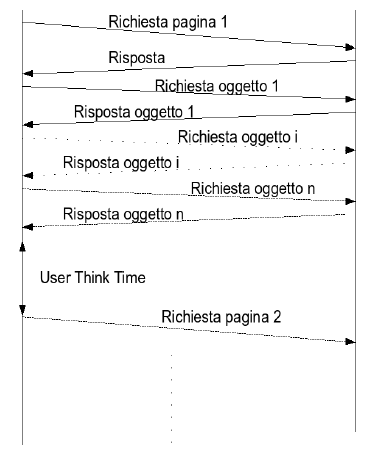
\includegraphics[scale=0.7]{etc/carico.png}
\caption{Carico}
\label{carico}
\end{center}
\end{figure}
Il singolo utente, durante una sessione, richiede un numero imprecisato di pagine web intervallate da un think time. Ognuna di queste pagine web può poi essere composta di oggetti embedded (nel caso in esame almeno due), come ad esempio fogli di stile, immagini e quant'altro. Di conseguenza il carico è stato generato seguendo quest'approccio:
\begin{enumerate}
	\item Si generano il numero di richieste per sessione che l'utente sottoporrà al sistema
	\item Si genera la dimensione della pagina da richiedere
	\item Si richiede ed ottiene il documento
	\item Si genera il numero di oggetti per la pagina richiesta
	\item Per ogni oggetto si genera la dimensione e si avvia la richiesta
	\item Si attende un tempo pari a User Think Time e se sono presenti altre richieste si torna al punto 2.
\end{enumerate}
Si presenta di seguito il frammento di codice rappresentante quest'approccio:
\begin{lstlisting}
//generazione delle sessioni e delle relative richieste 
while(i<array_length) { 
   session = session_request(mu_session, lambda_session); 
   for(j=0; j < session; j++) { 
        if( i < array_length) { 
           array[i] = html_page_size(mu_html, sigma_html, alfa_html); 	
       } 
   i++; 
   objects = object_per_request(alfa_obj); 
   for(k=0; k<objects; k++){ 
      if(i<array_length) 
          array[i] = embedded_object_size(mu_emb, sigma_emb); 
      i++; 
    } 
  } 
}
\end{lstlisting}

\section{Rappresentazione delle risorse}
Come brevemente introdotto in precedenza, una facility modella in ambiente CSIM una risorsa del sistema, con la rispettiva coda. La libreria mette a disposizione diversi tipologie di facility, scegliendo le più adatte al modello: 
\begin{itemize}
	\item facility risorsa con una sola coda ed un solo servente, occupabile da un solo processo alla volta; 
	\item facility set array di facility di primo tipo e quindi una risorsa con più code e più serventi (una coda per ogni servente) indipendenti tra loro. 
	\item multi-server facility risorsa con una sola coda ma più serventi, occupabili tutti contemporaneamente; 
\end{itemize}
Per realizzare la simulazione sono state utilizzate solo le prime due categorie. Si riporta il codice CSIM in cui avviene la dichiarazione delle suddette facility, che verranno analizzate in seguito:
\begin{lstlisting}
FACILITY cpuWS[NUM_SERVER]; 
FACILITY diskWS[NUM_DISK*NUM_SERVER]; 
FACILITY L2; 
FACILITY CPU_web_switch; 
FACILITY inLink; 
FACILITY outLink; 
FACILITY link_add; 
FACILITY LS1; 
FACILITY LS2; 
FACILITY LW2[NUM_SERVER]; 
FACILITY LW3[NUM_SERVER];
\end{lstlisting}
Prima di presentare le domande di servizio per ogni FACILITY, si definiscono dei parametri della rete e alcune funzioni di "supporto" per consentire una maggiore comprensione:
\begin{table}[H]
\begin{center}
\begin{tabular}{||c|c||}
\hline
\code{TCPOV} (overhead in byte introdotto dal TCP)						&20\\
\hline
\code{IPOV} (overhead in byte introdotto da IP)							&20\\
\hline
\code{FRAMEOV} (overhead in byte introdotto dal tipo di rete fisica)	&18\\
\hline
\code{MSS} (massima dimensione in byte di un pacchetto TCP)				&1460\\
\hline
\code{AVG\_SIZE\_HTTP\_REQ} (dimensione media di una richiesta HTTP)	&290\\
\hline
\end{tabular}
\end{center}
\caption{specifiche3}
\label{test_3}
\end{table}
\begin{lstlisting}
int NDatagrams(double m) { 
	int n; 
	double f; 
	f=m/(double)MSS;
	n=(int)ceil(f); 
	return n; 
} 
\end{lstlisting}
\code{Ndatagrams} consente di determinare il numero di messaggi necessari per inviare un messaggio lungo m bytes.
\begin{lstlisting}
int Overhead(double m) { 
   return (NDatagrams(m)*(TCPOV+IPOV+FRAMEOV)); 
}
\end{lstlisting}
\code{Overhead} rappresenta l'overhead necessario per inviare un messaggio lungo m bytes.
\begin{lstlisting}
double NetworkTime(double m, double bandwidth) { 
	return (double)(8*(m+Overhead(m)))/(double)(1000*1000*bandwidth); 
}
\end{lstlisting}
\code{NetworkTime} consente di calcolare il tempo (in secondi) necessario ad un messaggio lungo m bytes per transitare attraverso una rete caratterizzata da una banda \code{bandwidth} (in Mbps).
Si presentano di seguito le domande di servizio relative ai componenti della rete (N.B. : non sono presenti le domande di servizio delle schede di rete LS2, LW2 e LW3, poiché si è assunto che il loro transfer rate sia pari alla banda delle reti a cui sono collegate).
\begin{lstlisting}
double D_InLink() { 
    return NetworkTime(AVG_SIZE_HTTP_REQ, INLINK_BANDWIDTH) +    
    3*NetworkTime(0.0001, INLINK_BANDWIDTH); 
} 

double D_OutLink(double docSize) { 
    return NetworkTime(docSize, OUTLINK_BANDWIDTH) + 2 * NetworkTime(0.0001,   
    OUTLINK_BANDWIDTH); 
} 

double D_LAN(double docSize) { 
   if(docSize == 0) { 
       return NetworkTime(AVG_SIZE_HTTP_REQ, BANDWIDTH_L2); 
   } 
    return NetworkTime( docSize, BANDWIDTH_L2); 
} 
\end{lstlisting}
Per quanto concerne la domanda di servizio della LAN si è operata una distinzione tra fase di richieste (in cui \code{docSize = 0}) e fase di risposta
\begin{lstlisting}
double D_Cpu(double service_rate) { 
   return 1 / service_rate; 
}
\end{lstlisting}
La domanda di servizio della CPU vale sia per il Web Server che per il Web Switch, infatti il Service\_Rate dev'essere specificato come parametro di input.
\begin{lstlisting}
double D_WSDisk(double doc_size) { 
   double ret = (number_of_blocks(doc_size)) * ((DISK_SEEK_TIME/pow(10,3)) + ROTATIONAL_LATENCY + (CONTROLLER_TIME/pow(10,3)) + (BLOCK_SIZE/((double)DISK_TRANSFER_RATE*pow(10,6)))); 
   return ret; 
} 
\end{lstlisting}
La funzione \code{number\_of\_blocks} indica il numero di blocchi necessari da leggere per un intero documento di dimensione \code{doc\_size} bytes ed è così definita:
\begin{lstlisting}
int number_of_blocks(double docSize) { 
   return ceil(docSize/BLOCK_SIZE); 
}
\end{lstlisting}
I restanti parametri della domanda di servizio del disco sono:
\begin{description}
	\item[SeekTime:] secondi che impiega il braccio del disco a posizionarsi sul cilindro corretto 
	\item[ControllerTime:] secondi spesi dal controller del disco per processare una richiesta di I/O 
	\item[TransferRate:] tasso espresso in MB/sec con cui i dati vengono trasferiti dal/al disco 
	\item[BlockSize:] dimensione in bytes del blocco del disco 
	\item[RotationalLatency:] tempo medio in secondi affinchè il settore giusto capiti sotto la testina del braccio del disco 
\end{description}
\begin{lstlisting}
double D_linkAdd(double doc_size) { 
 return NetworkTime(doc_size, BANDWIDTH_LINKADD) + 2 * NetworkTime(0.0001, BANDWIDTH_LINKADD); 
} 

double D_LS1in() 
{ 
  return NetworkTime(AVG_SIZE_HTTP_REQ, LS1_TRANSFER_RATE) + 3*NetworkTime(0.0001, LS1_TRANSFER_RATE); 
} 

double D_LS1out(double doc_size) 
{ 
  return NetworkTime(doc_size, LS1_TRANSFER_RATE) + 2 * NetworkTime(0.0001, LS1_TRANSFER_RATE); 
}
\end{lstlisting}
\section{Dimensionamento del Sistema}
Rappresentato il workload e le risorse del sistema, è stato possibile dimensionare i parametri mancanti della rete, adottando un approccio di tipo empirico, iniziando a dimensionare i vari link per poi passare ai web server (CPU e Dischi). 
I parametri da dimensionare erano i seguenti:
\begin{itemize}
	\item Banda dell'incoming link;
	\item Banda dell'outgoing link;
	\item CPU Web Swtich Service Rate;
	\item Numero di Web Server
	\item Numero di dischi per Web Server
	\item Banda del link Addizionale
\end{itemize}
Transfer rate delle schede di rete LS1, LS2, LW2, LW3.
E' doveroso sottolineare che tutte le schede di rete sono state dimensionate tenendo conto delle reti a cui erano collegate e quindi queste presenteranno un transfer rate pari alla banda della LAN a cui sono accoppiate. Le simulazioni sono state condotte sulla configurazione standard del sistema in cui il server veniva scelto in modo random e  i risultati sono stati mediati su 10 run diversi, poiché non è molto corretto attenersi agli esiti di una singola simulazione del sistema. I parametri risultanti sono stati:
\begin{table}[H]
\begin{center}
\begin{tabular}{||c|c||}
\hline
Risorsa							&Valore\\
\hline
Banda incoming Link				&45 Mbps (T3)\\
\hline	
Banda Outgoing Link				&1000 Mbps\\
\hline
CPU Web Switch Service Rate		&9600 richieste/secondo\\
\hline
Numero di Web Server			&66\\
\hline
Numero di dischi per Web Server	&12\\
\hline
Transfer Rate LS1				&1000 Mbps\\
\hline
Transfer Rate LS2				&1000 Mbps\\
\hline
Transfer Rate lw2		&1000 Mbps\\
\hline
Transfer Rate LW3		&622 Mbps (OC-12)\\
\hline
Banda Link Addizionale	&622 Mbps (OC-12)\\
\hline
\end{tabular}
\end{center}
\caption{specifiche4}
\label{test_4}
\end{table}

\section{Transiente}
Un sistema web attraversa una fase iniziale durante la quale le code dei vari serventi cominciano a riempirsi, fino a raggiungere un livello di regime, in cui gli indici di prestazione del sistema assumono valori stabili. E’ quindi importante non tenere conto delle statistiche relative al periodo iniziale (transiente o transitorio), in quanto queste potrebbero rischiare di falsare i risultati complessivi. La determinazione della lunghezza del transiente è stata ricavata tramite l’algoritmo di Welch descritto da Law e Kelton in. Esso consente di determinare il numero di osservazioni l (di un indice del sistema Y ) che è necessario scartare dal numero totale di osservazioni m. Se l ed m sono scelti troppo piccoli la stima dell’indice potrebbe discostarsi 
dal caso stazionario; viceversa se l è scelto troppo grande la stima dell’indice rischia di possedere una varianza troppo grande. 
L’algoritmo proposto da Welch fa uso di una procedura grafica per determinare un valore di l tale che $E[Yi ] \approx lim(i \rightarrow \inf ) E[Y_{i}] = \nu per i > l $. Ciò è equivalente a determinare per quale valore di l la curva media del transiente si appiattisce fino a raggiungere il valore $\nu$ . In generale è difficile ricavare l tramite una singola replica, a causa della variabilità dell’indice Y. Per risolvere un tale problema Welch propone una procedura basata sull’utilizzo di n repliche della simulazione indipendenti tra loro. L'algoritmo è il seguente:
\begin{enumerate}
	\item Fare n repliche della simulazione ( dove $n\geq5$ ), ognuna di lunghezza m ( dove m sono le osservazioni fatte nella simulazione ), porre $Y_{ij}$ come la i-esima osservazione della j-esima replica ( $j = 1,2,\ldots,n; i = 1,2,\ldots ,m$ )
	\item Calcolare $Y_{i}$ come media delle $Y_{ij}$ di ogni replica
\begin{figure}[H]
\begin{center}
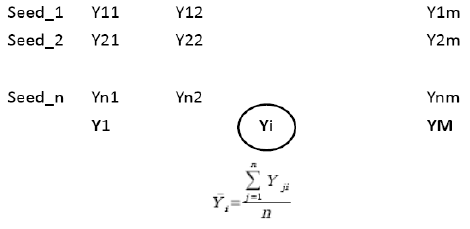
\includegraphics[scale=0.65]{etc/ipsilon.png}
\caption{Carico}
\label{carico}
\end{center}
\end{figure}
	\item Calcolare il valore di Moving average $Y_{i}(w)$, dove w è la finestra ed è un intero positivo tale che $w \leq \frac{m}{2}$, come segue: 
$$
Y_{w} = \lbrace{ \frac{\sum_{s=-w}^{w} Y_{i+s}}{2w+1} se i=w+1, \ldots,m-w }
$$
	\item Graficare la media mobile e si sceglie l = i tale che la media mobile sembra convergere.
\end{enumerate}
Per quanto riguarda il caso di studio in esame, sono state effettuate 3 prove utilizzando la configurazione standard (random), effettuando n=10 repliche della simulazione ognuna di lunghezza
m = 500000, graficando il tempo di risposta al variare della finestra W.

Caso 1: n=10, m = 500000, W = 5000
\begin{figure}[H]
\begin{center}
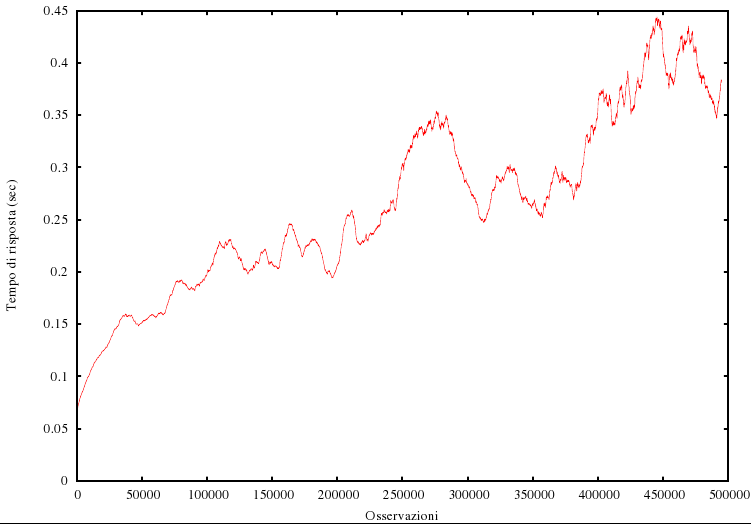
\includegraphics[scale=0.5]{etc/grafico1.png}
\caption{Grafico1}
\label{Grafico1}
\end{center}
\end{figure}
Utilizzando una finestra piccola rispetto al numero di osservazioni, si nota un'alta variabilità dei valori osservati e un trend monotono crescente all'aumentare del numero di osservazioni.

Caso2 : n=10, m=500000, W = 50000
\begin{figure}[H]
\begin{center}
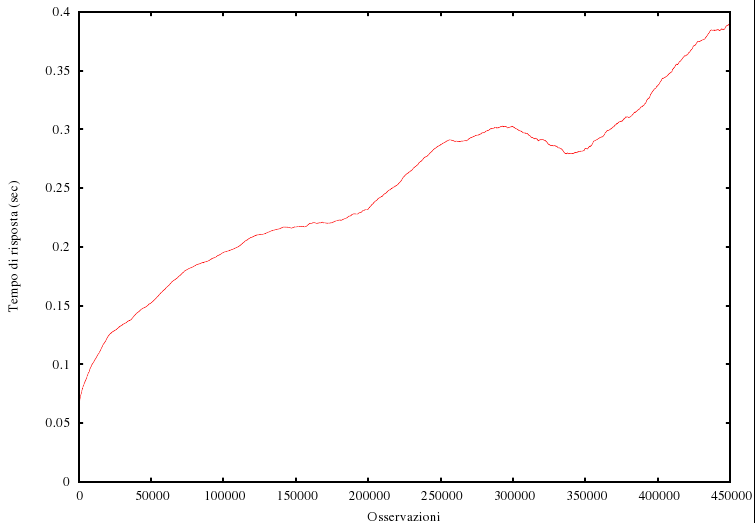
\includegraphics[scale=0.5]{etc/grafico2.png}
\caption{Grafico2}
\label{Grafico2}
\end{center}
\end{figure}
In questo caso è sempre presente l'andamento crescente del tempo di risposta, ma la variazione dei valori è molto minore rispetto al caso 1.

Caso3: n=10, m=500000, W = 100000
\begin{figure}[H]
\begin{center}
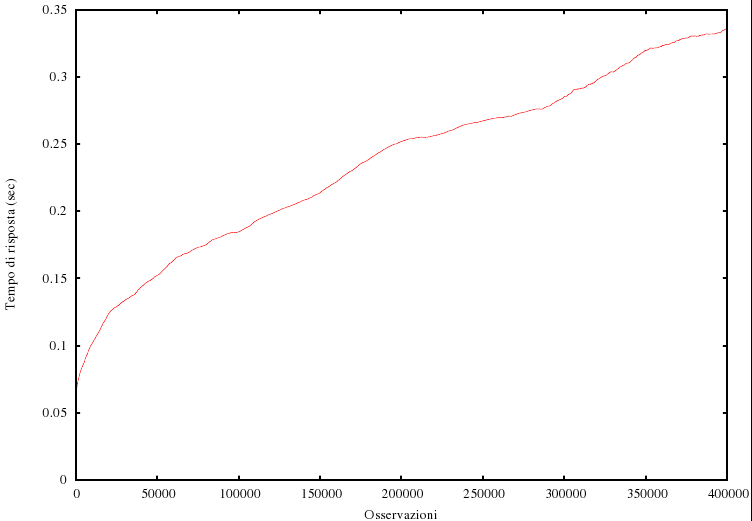
\includegraphics[scale=0.5]{etc/grafico3.png}
\caption{Grafico3}
\label{Grafico3}
\end{center}
\end{figure}
Anche in quest'ultimo caso, il tempo di risposta non sembra convergere, nonostante presenti un andamento piuttosto stabile. La mancata convergenza verso un valore potrebbe dipendere dalla distribuzione heavy tailed dei documenti, e dal fatto che i dischi potrebbero essere sottoposti a svolgere delle operazioni per file di centinaia di megabyte (si vedano i risultati del partizionamento del carico). Non essendo stato possibile determinare con precisione il valore l, si è deciso comunque  di eliminare dalla simulazione le prime 100000 osservazioni della simulazione, pur avendo la consapevolezza che il tempo di risposta tende ad aumentare al numero di osservazioni.

\section{Struttura della simulazione}
Si presentano di seguito alcuni aspetti ritenuti importanti per comprendere al meglio la simulazione, in modo particolare la generazione di una sessione e delle relative richieste (il processo web client), e il processo principale che si occupa di raccogliere le statistiche.
\subsection{Webclient}
Di seugito si riporta un frammento di codice relativo alla creazione di una sessione e relative richieste. 
\begin{lstlisting}
int session = session_request(mu_session, lambda_session); 
..
for(i=0; i < session; i++) { 
   html_page = html_page_size(mu_html, sigma_html, alfa_html); 
  set_process_class(requestClasses[get_doc_class(html_page)]); 
   if(variant == PROXY && stream_prob(p_hit_proxy) > 0.4) { 
     web_client(html_page, variant, bool_transient, iter); 
   } 
   if(variant != PROXY) { 
      web_client(html_page, variant, bool_transient, iter); 
   } 
   num_embedded_objects = object_per_request(alfa_obj); 
   for(j=0; j < num_embedded_objects; j++) { 
      emb_obj_size = embedded_object_size(mu_emb, sigma_emb); 
      set_process_class(requestClasses[get_doc_class(emb_obj_size)]); 
      if(variant == PROXY && stream_prob(p_hit_proxy) > 0.4) { 
          web_client(emb_obj_size, variant, bool_transient, iter); 
     } 
     if(variant != PROXY) { 
         web_client(emb_obj_size, variant, bool_transient, iter); 
     } 
  } 
  hold(user_think_time(alfa_tt));
}
\end{lstlisting}
Per ogni richiesta della sessione viene invocata la funzione web\_client specifica quali risorse vengono utilizzate e in che misura. 
\begin{figure}[H]
\begin{center}
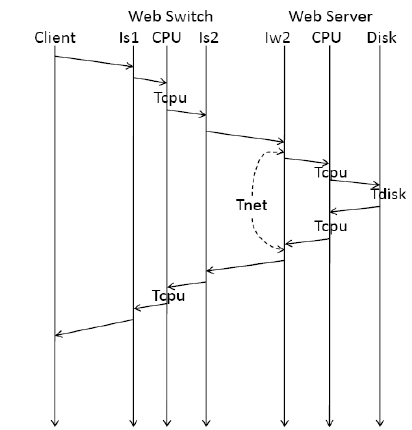
\includegraphics[scale=0.62]{etc/webclient.png}
\caption{webclient}
\label{webclient}
\end{center}
\end{figure}
\begin{figure}[H]
\begin{center}
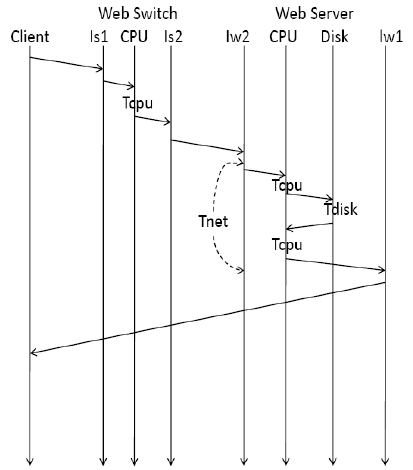
\includegraphics[scale=0.62]{etc/webclient2.png}
\caption{webclient2}
\label{webclient2}
\end{center}
\end{figure}

Si presenta di seguito un frammento della funzione web\_client per specificare come avvengono i cicli di richiesta risposta sopra rappresentati. In CSIM questi cicli sono rappresentati da un uso esclusivo delle risorse modellate: 
\begin{lstlisting}
use(inLink, D_InLink()); 
switch_start_time = enter_box(WebSwitch); 
use(LS1, D_LS1in()); 
use(CPU_web_switch, D_Cpu(CPU_WEB_SWITCH_SERVICE_RATE)); 
 use(LS2, D_LAN(0)); //stessa banda della LAN, in richiesta doc_size=0 
 exit_box(WebSwitch, switch_start_time); 
 use(L2, D_LAN(0)); 
/* random */ 
if(variant == RANDOM || variant == LINK_ADD || variant == PROXY) { 
    tmp_server = current_server; 
    current_server = csim_random_int(0, NUM_SERVER-1); 
} 
else if (variant == ROUND_ROBIN) { //round robin 
    tmp_server = current_server; 
    current_server = (tmp_server+1)%NUM_SERVER; 
} 
// least loaded 
else if (variant == LEAST_LOADED) { 
   tmp_server = get_least_loaded(); 
} 
server_start_time = enter_box(WebServer); 
use(LW2[tmp_server], D_LAN(0)); 
use(cpuWS[tmp_server], D_Cpu(CPU_SERVICE_RATE)); 
//selezione del disco round robin 
tmp_disk = currentDisk[tmp_server]; 
currentDisk[tmp_server] = (tmp_disk+1)%NUM_DISK; 
use(diskWS[tmp_server*NUM_DISK + tmp_disk], D_WSDisk(doc_size)); 
use(cpuWS[tmp_server], D_Cpu(CPU_SERVICE_RATE)); 
if(variant != LINK_ADD) { 
    use(LW2[tmp_server], D_LAN(doc_size)); 
} 
else { 
   use(LW3[tmp_server], D_linkAdd(doc_size)); 
}		 
exit_box(WebServer, server_start_time); 
if(variant == LINK_ADD) { 
   use(link_add, D_linkAdd(doc_size)); 
}		  
else { 
  use(L2, D_LAN(doc_size)); 
  use(LS2, D_LAN(doc_size)); 
  use(CPU_web_switch, D_Cpu(CPU_WEB_SWITCH_SERVICE_RATE)); 
  use(LS1, D_LS1out(doc_size)); 
  use(outLink, D_OutLink(doc_size)); 
}	
\end{lstlisting}
Dal frammento di codice sopra riportato si può notare come sia il web switch che i web server sono stati modellati attraverso dei BOXES (che servono per collezionare statistiche relative ad un sottoinsieme delle risorse di un sistema), inoltre si può notare come alcuni componenti nel caso sia presente il link addizionale siano molto meno utilizzati (come ad esempio il web switch o la LAN L2).

\subsection{Il processo principale}
Ogni client è rappresentato come appena discusso da un processo CSIM. Ogni processo viene 
creato da un processo principale secondo una particolare legge degli arrivi (in questo caso 
esponenziale). Il processo principale si occupa inoltre di reimpostare le statistiche raccolte una volta 
superato il periodo di transiente in maniera da escludere dalle considerazioni finali quelli che sono valori non particolarmente aderenti alla realtà perché ottenuti in condizioni del sistema non standard (carico minino, code vuote etc.). 
La simulazione procede, grazie al costrutto while e la condizione di convergenza, finché non 
vengono raccolti valori tali da ottenere dei risultati considerati rilevanti (con un certo grado di confidenza) Nel caso in esame si è scelto un livello di confidenza del 98\% con un errore relativo  di 0.005.
Il codice che realizza tutto questo è di seguito riportato. 
\begin{lstlisting}
..
for(i=0; i<NUM_ITERATIONS; i++){
 ...
 while(state(converged)==NOT_OCC && num_osservazioni<500000) { 
   hold(exponential(1/(double)ARRIVAL)); 
   web_session(client_id, variante, 0, -1); 
   client_id++; 
   //valori da scartare perche' facenti parte del transiente
   if(num_osservazioni>100000 &&(!reset)) { 
       printf("Reset statistics %g\n", simtime()); 
       reset(); 
       reset=1; 
       ...
   } 
} 
report_facilities(); 
report_table(rtime); 
report_boxes(); 
meter_summary(); 
tabulate(resptime, table_mean(rtime)); 
statistics(i, variante); 
rerun();
...
}
\end{lstlisting}
Dal frammento di codice sopra riportato si può notare il ciclo \code{for} e la funzione \code{rerun()} che consentono di eseguire più simulazioni e quindi di ottenere risultati più accurati; inoltre si può notare come siano stati scartati i valori relativi al transiente. E' opportuno sottolineare come alla condizione di convergenza sia stata aggiunta un'ulteriore condizione basata sul numero di osservazioni, poiché come visto nello studio del transiente, la convergenza potrebbe non verificarsi per tutte le iterazioni.

\section{Presentazione dei risultati}
Si presentano di seguito i risultati mediati su 10 iterazioni, per ogni componente del sistema preso in esame e per tutte le varianti analizzate. Le statistiche riportate sono l'utilizzazione, la lunghezza media delle coda e il tempo di risposta per ogni classe di richiesta.
\subsection{Risultati Random}
\begin{table}[H]
\begin{center}
\begin{tabular}{||c|c|c|c|c||}
\hline
Utilizzazioni\\
\hline
Centro &Classe1 &Classe2 &Classe3 &Totale\\
\hline
\hline
 cpu web server i-esimo: 	&0.6673596	&0.0000002	&0.0000001	&0.6673599\\
\hline
 disco i-esimo: 	&0.2901815	&0.0000000	&0.0000000	&0.2901815\\
\hline
 inLink: 	&0.3070558	&0.0000002	&0.0000001	&0.3070561\\
\hline
 outLink: 	&0.2779962	&0.0000000	&0.0000000	&0.2779962\\
\hline
 cpu web switch: 	&0.6882190	&0.0000003	&0.0000001	&0.6882193\\
\hline
 LAN: 	&0.2774720	&0.0000000	&0.0000000	&0.2774720\\
\hline
 LS1: 	&0.2917997	&0.0000000	&0.0000000	&0.2917997\\
\hline
 LS2:	&0.2774737	&0.0000000	&0.0000000	&0.2774737\\
\hline
 LW2: 	0.0042041	0.0000000	0.0000000	&0.0042041\\
\hline
\end{tabular}
\end{center}
\caption{Utilizzazioni}
\label{risrandom}
\end{table}
Come si può notare, il vincolo sull'utilizzazione richiesto nelle specifiche del progetto è stato rispettato, con la risorsa collo di bottiglia (CPU Web Switch) che presenta un'utilizzazione del 68,8\%. Le altre risorse, ad eccezione della CPU del web server, presentano un'utilizzazione piuttosto basse.

\begin{table}[H]
\begin{center}
\begin{tabular}{||c|c|c|c|c||}
\hline
Lunghezza media delle code\\
\hline
Centro &Classe1 &Classe2 &Classe3 &Totale\\
\hline
\hline
 cpu web server i-esimo: 	&1.5556346	&0.0000003	&0.0000001	&1.5556350\\
\hline
 disco i-esimo: 	&1.6398481	&0.0000002	&0.0000000	&1.6398483\\
\hline
 inLink: 	&0.8287492	&0.0000002	&0.0000001	&0.8287495\\
\hline
 outLink: 	&4.2762899	&0.0000000	&0.0000000	&4.2762899\\
\hline
 cpu web switch: 	&3.6788684	&0.0000005	&0.0000003	&3.6788692\\
\hline
 LAN: 	&1.6334769	&0.0000001	&0.0000000	&1.6334770\\
\hline
 LS1: 	&3.3884849	&0.0000000	&0.0000000	&3.3884849\\
\hline
 LS2: 	&2.7263059	&0.0000002	&0.0000001	&2.7263062\\
\hline
 LW2: 	&0.0044529	&0.0000000	&0.0000000	&0.0044529\\
\hline
\end{tabular}
\end{center}
\caption{Lunghezza code}
\label{ris}
\end{table}
Per quanto concerne la lunghezza della coda, si nota un accodamento delle risposte nel link di uscita, che presenta valori più alti persino del web switch.
\begin{table}[htbp]
\caption{Tempo medio di risposta}
\begin{center}
\begin{tabular}{|c|c|c|c|}
\hline
Tempo Medio di Risposta\\
\hline
Centro &Classe1 &Classe2 &Classe3\\
\hline
\hline
 cpu web server i-esimo: 	&0.0155025	&0.0000349	&0.0000133\\
\hline
 disco i-esimo: 	&0.8416113	&0.0000000	&0.0000000\\
\hline
 inLink: 	&0.0002501	&0.0000286	&0.0000122\\
\hline
 outlink: 	&0.0012935	&0.0000000	&0.0000000\\
\hline
 cpu web switch: 	&0.0005546	&0.0000599	&0.0000377\\
\hline
 LAN: 	&0.0002467	&0.0000079	&0.0000003\\
\hline
 LS1: 	&0.0005116	&0.0000013	&0.0000004\\
\hline
 LS2: 	&0.0004116	&0.0000223	&0.0000111\\
\hline
 LW2: 	&0.0000445	&0.0000000	&0.0000000\\
\hline
\end{tabular}
\end{center}
\label{tempomediorisposta}
\end{table}
I tempi medi di risposta per la Classe1 evidenziano una lentezza generale dei dischi nel soddisfare le richieste. Per le altre due classi non è possibile fare alcun tipo di assunzione, dato il limitato numero di osservazioni di Classi 2 e 3 a cui è sottoposto il sistema e dato il limite temporale della simulazione, che non permette alle richieste di queste due classi di essere soddisfatte (non mi piace molto la cosa del limitato numero di osservazioni). Risultati sicuramente più significativi per le Classi superiori saranno osservabili nel momento in cui verranno presentati i risultati del modello analitico.

\subsection{Risultati Round Robin}
\begin{table}[htbp]
\begin{center}
\begin{tabular}{|c|c|c|c|c|}
\hline
Utilizzazioni\\
\hline
Centro &Classe1 &Classe2 &Classe3 &Totale\\
\hline
\hline
 cpu web server i-esimo: 	&0.6747827	&0.0000003	&0.0000001	&0.6747830\\
\hline
 disco i-esimo: 	&0.2937349	&0.0000000	&0.0000000	&0.2937349\\
\hline
 inLink: 	&0.3104327	&0.0000002	&0.0000001	&0.3104331\\
\hline
 outLink: 	&0.2814336	&0.0000000	&0.0000000	&0.2814336\\
\hline
 cpu web switch: 	&0.6958719	&0.0000003	&0.0000001	&0.6958723\\
\hline
 LAN: 	&0.2809161	&0.0000000	&0.0000000	&0.2809161\\
\hline
 LS1: 	&0.2954094	&0.0000000	&0.0000000	&0.2954094\\
\hline
 LS2:	&0.2809159	&0.0000000	&0.0000000	&0.2809159\\
\hline
 LW2: 	0.0042562	0.0000000	0.0000000	&0.0042562\\
\hline
\end{tabular}
\end{center}
\caption{Utilizzazioni}
\label{utilizzazioni}
\end{table}
Le utilizzazioni delle varie risorse adottando la politica round robin sono quasi identiche a quelle con politica random presentate precedentemente.
\begin{table}[htbp]
\begin{center}
\begin{tabular}{|c|c|c|c|c|}
\hline
Lunghezza media delle code\\
\hline
Centro &Classe1 &Classe2 &Classe3 &Totale\\
\hline
\hline
 cpu web server i-esimo: 	&1.0056119	&0.0000004	&0.0000001	&1.0056125\\
\hline
 disco i-esimo: 	&1.6242344	&0.0000000	&0.0000002	&1.6242346\\
\hline
 inLink: 	&0.8558574	&0.0000002	&0.0000005	&0.8558581\\
\hline
 outLink: 	&4.4133256	&0.0000000	&0.0000000	&4.4133256\\
\hline
 cpu web switch: 	&3.9749297	&0.0000004	&0.0000003	&3.9749304\\
\hline
 LAN: 	&1.6945618	&0.0000001	&0.0000000	&1.6945619\\
\hline
 LS1: 	&3.4855153	&0.0000006	&0.0000000	&3.4855159\\
\hline
 LS2: 	&2.8162152	&0.0000000	&0.0000001	&2.8162153\\
\hline
 LW2: 	&0.0045441	&0.0000000	&0.0000000	&0.0045441\\
\hline
\end{tabular}
\end{center}
\caption{Lunghezza Code}
\label{lunghezzacode}
\end{table}
Rispetto al caso presentato precedentemente, si nota un leggero aumento delle code dei dischi del web server e della cpu del web switch, mentre si ha una leggera diminuzione o valori analoghi per tutte le altre risorse.
\begin{table}[htbp]
\begin{center}
\begin{tabular}{|c|c|c|c|}
\hline
Tempo Medio di Risposta\\
\hline
Centro &Classe1 &Classe2 &Classe3\\
\hline
\hline
 cpu web server i-esimo: 	&0.0099264	&0.0000537	&0.0000101\\
\hline
 disco i-esimo: 	&0.5745555	&0.0000000	&0.0000000\\
\hline
 inLink: 	&0.0002556	&0.0000278	&0.0000574\\
\hline
 outlink: 	&0.0013225	&0.0000000	&0.0000000\\
\hline
 cpu web switch: 	&0.0005932	&0.0000531	&0.0000403\\
\hline
 LAN: 	&0.0002535	&0.0000113	&0.0000003\\
\hline
 LS1: 	&0.0005215	&0.0000742	&0.0000004\\
\hline
 LS2: 	&0.0004213	&0.0000008	&0.0000151\\
\hline
 LW2: 	&0.0000449	&0.0000000	&0.0000000\\
\hline
\end{tabular}
\end{center}
\caption{Tempo medio di risposta}
\label{tempomediorisposta}
\end{table}
Anche per quanto riguarda i tempi medi di risposta, i risultati sono analoghi al caso precedente, fatta eccezione per i dischi del web server che presentano un leggero aumento dei tempi, dovuti all'aumento delle code.
\subsection{Risultati Least Loaded}
\begin{table}[htbp]
\begin{center}
\begin{tabular}{|c|c|c|c|c|}
\hline
Utilizzazioni\\
\hline
Centro &Classe1 &Classe2 &Classe3 &Totale\\
\hline
\hline
 cpu web server i-esimo: 	&0.7167869	&0.0000002	&0.0000001	&0.7167871\\
\hline
 disco i-esimo: 	&0.3128002	&0.0000000	&0.0000000	&0.3128002\\
\hline
 inLink: 	&0.3294591	&0.0000002	&0.0000001	&0.3294594\\
\hline
 outLink: 	&0.2996635	&0.0000000	&0.0000000	&0.2996635\\
\hline
 cpu web switch: 	&0.7392626	&0.0000002	&0.0000001	&0.7392628\\
\hline
 LAN: 	&0.2990815	&0.0000000	&0.0000000	&0.2990815\\
\hline
 LS1: 	&0.3144901	&0.0000000	&0.0000000	&0.3144901\\
\hline
 LS2:	&0.2990815	&0.0000000	&0.0000000	&0.2990815\\
\hline
 LW2: 	0.0045316	0.0000000	0.0000000	&0.0045316\\
\hline
\end{tabular}
\end{center}
\caption{Utilizzazioni}
\label{utilizzazioni}
\end{table}
Adottando questa politica diminuiscono i tempi medi di servizio e di conseguenza si ha un aumento del carico del sistema. Per questo motivo è possibile notare un aumento delle utilizzazioni per tutte le risposte del sistema, che porta a superare la soglia del 70\% sia per la CPU del web switch che per quella del Web Server.
\begin{table}[htbp]
\begin{center}
\begin{tabular}{|c|c|c|c|c|}
\hline
Lunghezza media delle code\\
\hline
Centro &Classe1 &Classe2 &Classe3 &Totale\\
\hline
\hline
 cpu web server i-esimo: 	&3.9782364	&0.0000012	&0.0000006	&3.9782382\\
\hline
 disco i-esimo: 	&0.6957288	&0.0000000	&0.0000000	&0.6957288\\
\hline
 inLink: 	&1.0129555	&0.0000002	&0.0000001	&1.0129558\\
\hline
 outLink: 	&5.6197781	&0.0000000	&0.0000000	&5.6197781\\
\hline
 cpu web switch: 	&6.0216761	&0.0000009	&0.0000001	&6.0216771\\
\hline
 LAN: 	&2.0022744	&0.0000002	&0.0000000	&2.0022746\\
\hline
 LS1: 	&4.5046757	&0.0000000	&0.0000000	&4.5046757\\
\hline
 LS2: 	&3.6126354	&0.0000000	&0.0000000	&3.6126354\\
\hline
 LW2: 	&0.0051400	&0.0000000	&0.0000000	&0.0051400\\
\hline
\end{tabular}
\end{center}
\caption{Lunghezza Code}
\label{lunghezzacode}
\end{table}
Come avviene per le utilizzazioni, anche la lunghezza media delle code aumenta per tutti i centri, ad eccezione dei dischi del web server, poiché non accade mai che un server particolarmente carico riceva altre richieste da far processare ai suoi dischi se prima le code non sono state svuotate
\begin{table}[htbp]
\begin{center}
\begin{tabular}{|c|c|c|c|}
\hline
Tempo Medio di Risposta\\
\hline
Centro &Classe1 &Classe2 &Classe3\\
\hline
\hline
 cpu web server i-esimo: 	&0.0365676	&0.0001307	&0.0000703\\
\hline
 disco i-esimo: 	&0.1738966	&0.0000000	&0.0000000\\
\hline
 inLink: 	&0.0002853	&0.0000227	&0.0000093\\
\hline
 outlink: 	&0.0015856	&0.0000000	&0.0000000\\
\hline
 cpu web switch: 	&0.0008480	&0.0000995	&0.0000137\\
\hline
 LAN: 	&0.0002824	&0.0000231	&0.0000003\\
\hline
 LS1: 	&0.0006352	&0.0000008	&0.0000004\\
\hline
 LS2: 	&0.0005094	&0.0000005	&0.0000003\\
\hline
 LW2: 	&0.0000495	&0.0000000	&0.0000000\\
\hline
\end{tabular}
\end{center}
\caption{Tempo medio di risposta}
\label{tempomediodirisposta}
\end{table}
I tempi di risposta sono più o meno analoghi a quelli presentati in precedenza, fatta eccezione per i dischi del web server, che, come ci si poteva aspettare, riducono il loro tempo medio di risposta.
\subsection{Risultati Proxy}
\begin{table}[htbp]
\begin{center}
\begin{tabular}{|c|c|c|c|c|}
\hline
Utilizzazioni\\
\hline
Centro &Classe1 &Classe2 &Classe3 &Totale\\
\hline
\hline
 cpu web server i-esimo: 	&0.4382355	&0.0000001	&0.0000000	&0.4382356\\
\hline
 disco i-esimo: 	&0.1921759	&0.0000000	&0.0000000	&0.1921759\\
\hline
 inLink: 	&0.2014804	&0.0000001	&0.0000000	&0.2014805\\
\hline
 outLink: 	&0.1842500	&0.0000000	&0.0000000	&0.1842500\\
\hline
 cpu web switch: 	&0.4519287	&0.0000001	&0.0000000	&0.4519288\\
\hline
 LAN: 	&0.1838706	&0.0000000	&0.0000000	&0.1838706\\
\hline
 LS1: 	&0.1933170	&0.0000000	&0.0000000	&0.1933170\\
\hline
 LS2:	&0.1838711	&0.0000000	&0.0000000	&0.1838711\\
\hline
 LW2: 	0.0027859	0.0000000	0.0000000	&0.0027859\\
\hline
\end{tabular}
\end{center}
\caption{Utilizzazioni}
\label{utilizzazioni}
\end{table}
L'introduzione del proxy, con un cache hit rate del 40\%, porta ad un notevole calo delle utilizzazioni, riducendo a meno del 46\% l'utilizzazione della risorsa collo di bottiglia del sistema (la CPU del web switch) e della CPU del Web Server. 
\begin{table}[htbp]
\begin{center}
\begin{tabular}{|c|c|c|c|c|}
\hline
Lunghezza media delle code\\
\hline
Centro &Classe1 &Classe2 &Classe3 &Totale\\
\hline
\hline
 cpu web server i-esimo: 	&0.6329342	&0.0000002	&0.0000000	&0.6329343\\
\hline
 disco i-esimo: 	&0.9622401	&0.0000000	&0.0000000	&0.9622401\\
\hline
 inLink: 	&0.3370955	&0.0000001	&0.0000000	&0.3370956\\
\hline
 outLink: 	&2.1766564	&0.0000000	&0.0000000	&2.1766564\\
\hline
 cpu web switch: 	&0.9132859	&0.0000002	&0.0000000	&0.9132861\\
\hline
 LAN: 	&0.8057551	&0.0000000	&0.0000000	&0.8057551\\
\hline
 LS1: 	&1.7810221	&0.0000057	&0.0000000	&1.7810278\\
\hline
 LS2: 	&1.3518652	&0.0000001	&0.0000000	&1.3518653\\
\hline
 LW2: 	&0.0029656	&0.0000000	&0.0000000	&0.0029656\\
\hline
\end{tabular}
\end{center}
\caption{Lunghezza Code}
\label{lunghezzacode}
\end{table}
Anche le code tendono a diminuire notevolmente, come era logico aspettarsi. 
\begin{table}[htbp]
\begin{center}
\begin{tabular}{|c|c|c|c|}
\hline
Tempo Medio di Risposta\\
\hline
Centro &Classe1 &Classe2 &Classe3\\
\hline
\hline
 cpu web server i-esimo: 	&0.0096208	&0.0000288	&0.0000000\\
\hline
 disco i-esimo: 	&1.0033886	&0.0000000	&0.0000000\\
\hline
 inLink: 	&0.0001552	&0.0000186	&0.0000000\\
\hline
 outlink: 	&0.0010055	&0.0000000	&0.0000000\\
\hline
 cpu web switch: 	&0.0002102	&0.0000291	&0.0000000\\
\hline
 LAN: 	&0.0001859	&0.0000005	&0.0000000\\
\hline
 LS1: 	&0.0004110	&0.0011045	&0.0000000\\
\hline
 LS2: 	&0.0003119	&0.0000110	&0.0000000\\
\hline
 LW2: 	&0.0000451	&0.0000000	&0.0000000\\
\hline
\end{tabular}
\end{center}
\caption{Tempo medio di risposta}
\label{tempomediodirisposta}
\end{table}
Analogo discorso vale anche per i tempi medi di risposta. Si ricorda che per l'esecuzione della simulazione con l'introduzione del proxy (e con il link addizionale, che sarà presentato nella prossima  sezione), è stata adottata la politica random.

\subsection{Risultati Link Addizionale}
\begin{table}[htbp]
\begin{center}
\begin{tabular}{|c|c|c|c|c|}
\hline
Utilizzazioni\\
\hline
Centro &Classe1 &Classe2 &Classe3 &Totale\\
\hline
\hline
 cpu web server i-esimo: 	&0.6729036	&0.0000003	&0.0000001	&0.6729039\\
\hline
 disco i-esimo: 	&0.2926927	&0.0000000	&0.0000000	&0.2926927\\
\hline
 inLink: 	&0.3096163	&0.0000002	&0.0000001	&0.3096167\\
\hline
 outLink: 	&0.0000000	&0.0000000	&0.0000000	&0.0000000\\
\hline
 cpu web switch: 	&0.3475399	&0.0000003	&0.0000001	&0.3475402\\
\hline
 LAN: 	&0.0090708	&0.0000000	&0.0000000	&0.0090708\\
\hline
 LS1: 	&0.0139327	&0.0000000	&0.0000000	&0.0139327\\
\hline
 LS2:	&0.0090708	&0.0000000	&0.0000000	&0.0090708\\
\hline
 LW2: 	0.0001374	0.0000000	0.0000000	&0.0001374\\
\hline
 LINK_ADD: 	&0.4508218	&0.0000000	&0.0000000	&0.4508218\\
\hline
 LW3: 	&0.0068306	&0.0000000	&0.0000000	&0.0068306\\
\hline
\end{tabular}
\end{center}
\caption{Utilizzazioni}
\label{utilizzazioni}
\end{table}
L'introduzione del link addizionale comporta una notevole diminuzione dell'utilizzazione della cpu del web switch e  della maggior parte delle componenti di rete, come la LAN L2 e le schede di rete LS1, LS2 e LW2, poiché queste hanno il compito di gestire solamente le richieste, mentre le risposte  vengono interamente smistate verso la scheda di rete LW3 e il link addizionale.
\begin{table}[htbp]
\begin{center}
\begin{tabular}{|c|c|c|c|c|}
\hline
Lunghezza media delle code\\
\hline
Centro &Classe1 &Classe2 &Classe3 &Totale\\
\hline
\hline
 cpu web server i-esimo: 	&1.5404288	&0.0000006	&0.0000001	&1.5404295\\
\hline
 disco i-esimo: 	&1.6460958	&0.0000006	&0.0000000	&1.6460963\\
\hline
 inLink: 	&0.4752640	&0.0000007	&0.0000001	&0.4752647\\
\hline
 outLink: 	&0.0000000	&0.0000000	&0.0000000	&0.0000000\\
\hline
 cpu web switch: 	&0.4067200	&0.0000004	&0.0000001	&0.4067205\\
\hline
 LAN: 	&0.0090708	&0.0000000	&0.0000000	&0.0090708\\
\hline
 LS1: 	&0.0139327	&0.0000000	&0.0000000	&0.0139327\\
\hline
 LS2: 	&0.0090708	&0.0000000	&0.0000000	&0.0090708\\
\hline
 LW2: 	&0.0001374	&0.0000000	&0.0000000	&0.0001374\\
\hline
 LINK_ADD: 	&3.5259678	&0.0000000	&0.0000000	&3.5259678\\
\hline
 LW3: 	&0.0071490	&0.0000000	&0.0000000	&0.0071490\\
\hline
\end{tabular}
\end{center}
\caption{Lunghezza Code}
\label{lunghezzacode}
\end{table}
Anche la lunghezza media delle code dello switch e delle componenti di rete tende a diminuire notevolmente, mentre restano immutate quelle dei web server.
\begin{table}[htbp]
\begin{center}
\begin{tabular}{|c|c|c|c|}
\hline
Tempo Medio di Risposta\\
\hline
Centro &Classe1 &Classe2 &Classe3\\
\hline
\hline
 cpu web server i-esimo: 	&0.0152177	&0.0000734	&0.0000101\\
\hline
 disco i-esimo: 	&0.8363018	&0.0000000	&0.0000000\\
\hline
 inLink: 	&0.0001423	&0.0000773	&0.0000093\\
\hline
 outlink: 	&0.0000000	&0.0000000	&0.0000000\\
\hline
 cpu web switch: 	&0.0001219	&0.0000428	&0.0000104\\
\hline
 LAN: 	&0.0000027	&0.0000008	&0.0000003\\
\hline
 LS1: 	&0.0000042	&0.0000013	&0.0000004\\
\hline
 LS2: 	&0.0000027	&0.0000008	&0.0000003\\
\hline
 LW2: 	&0.0000027	&0.0000000	&0.0000000\\
\hline
 LINK_ADD: 	&0.0010579	&0.0000000	&0.0000000\\
\hline
 LW3: 	&0.0001419	&0.0000000	&0.0000000\\
\hline
\end{tabular}
\end{center}
\caption{Tempo medio di risposta}
\label{tempomediodirisposta}
\end{table}
Quanto evidenziato in precedenza, risulta essere valido anche per il tempo medio di risposta.
